\documentclass[a4paper,12pt]{report}
\usepackage[left=2cm,right=2cm,top=2cm,bottom=2cm]{geometry}
\usepackage[utf8]{inputenc}
\usepackage{graphicx}
\usepackage{eso-pic}
\usepackage{transparent}
\usepackage{xcolor}
\usepackage{floatrow}
\usepackage{tabularx}
\usepackage{listings}
\usepackage{xcolor}
\usepackage{caption}

\newcommand{\LogoPath}{RUET_logo.png}

\definecolor{odp-background}{RGB}{40, 44, 52}
\definecolor{odp-text}{RGB}{171, 178, 191}
\definecolor{odp-keyword}{RGB}{249, 38, 114}
\definecolor{odp-comment}{RGB}{98, 114, 164}
\definecolor{odp-string}{RGB}{152, 195, 121}
\definecolor{odp-number}{RGB}{174, 129, 255}
\definecolor{odp-function}{RGB}{189, 147, 249}

\lstdefinestyle{cppstyle}{
    language=C++,
    basicstyle=\color{odp-text}\ttfamily\small,
    keywordstyle=\color{odp-keyword},
    commentstyle=\color{odp-comment},
    stringstyle=\color{odp-string},
    numbers=left,
    numberstyle=\tiny\color{odp-number},
    stepnumber=1,
    numbersep=5pt,
    backgroundcolor=\color{gray!5},
    frame=single,
    rulecolor=\color{odp-text},
    breaklines=true,
    breakatwhitespace=true,
    tabsize=4,
    moredelim=[s][\color{odp-header}]{\#include\ <}{>}, % Header files included in #include <>
    otherkeywords={!,!=,~,$,*,\&,\%,:,\#, ifndef, define, endif, include},
    emph={!,!=,~,$,*,\&,\%,:,\#},
    emphstyle=\color{odp-function}
}

\begin{document}
\begin{titlepage}
    \begin{center}

        \AddToShipoutPicture*{\put(0.125\paperwidth,0.125\paperheight){
                \transparent{0.1}
                \includegraphics*[width=0.75\paperwidth,height=0.75\paperheight,keepaspectratio]{RUET_logo.png}%
            }
        }
        \textbf{\textcolor{yellow}{\rmfamily Haven's Light is Our Guide}}

        \begin{figure}[h]
            \transparent{0.8}
            \centering
            \includegraphics[width=0.3\textwidth]{\LogoPath}
        \end{figure}

        \vspace*{0in}
        \Large
        \textbf{\mbox{Rajshahi University of Engineering \& Technology}}
        \large
        \textbf{\mbox{\textcolor{blue}{Department of Computer Science \& Engineering}}}

        \vfill
        \Huge
        \textbf{\mbox{Lab Report}}
        \vfill

        \begin{table}[h]
            \centering
            \begin{tabularx}{0.7\paperwidth}{|c|X|}
                \hline
                \textbf{Course Code:}     & CSE 2204                                                                         \\
                \hline
                \textbf{Course Title:}    & Numerical Methods Sessional                                                      \\
                \hline
                \textbf{Experiment No:}   & 04                                                                               \\
                \hline
                \textbf{Experiment Name:} & Find the straight line that best fits some given data using Least Square Method. \\
                \hline
            \end{tabularx}
        \end{table}

        \vspace{0.5in}
        \textbf{Date:} \\
        \today

        \vfill

        \begin{table}[h]
            \centering
            \begin{tabularx}{0.7\paperwidth}{|X|X|}
                \hline
                Submitted By:               & Submitted To:                                    \\
                \hline
                Name: Md. Abdullah Al Mamun & Shyla Afroge                                     \\
                \hline
                Section: A                  & Assistant Professor                              \\
                \hline
                Roll No: 2003028            & Computer Science \& Engineering                  \\
                \hline
                Year: 2nd Year Odd Semester & Rajshahi University of Engineering \& Technology \\
                \hline
            \end{tabularx}
        \end{table}
    \end{center}
\end{titlepage}

\section*{Experiment No: 04}
\section*{Experiment Name: \small Find the straight line that best fits some given data using Least Square Method.}
\section*{Theory:}

\subsection*{Least Square Method:}
\qquad The least squares method is a statistical technique used to determine the optimal parameters of a linear regression model by minimizing the sum of the squared differences between observed and predicted values. It aims to find the coefficients (intercept $a_0$ and slope $a_1$) that minimize the overall squared residuals in the data. The optimization involves solving the normal equations, resulting in formulas for $a_0$ and $a_1$ that provide the best-fitting line. This method is widely applied in various fields for modeling and predicting relationships between variables, as it provides a systematic way to estimate parameters that yield the most accurate linear approximation to the given data.

\subsection*{Algorithm:}
Given a set of data points $ (x_i, y_i) $ for $ i = 1, 2, \ldots, n $:

\begin{enumerate}
    \item Formulate the linear regression model: $ Y = a_0 + a_1x + \varepsilon $, where $ Y $ is the dependent variable, $ x $ is the independent variable, and $ \varepsilon $ is the error term.
    \item Define the cost function: $ J(a_0, a_1) = \sum_{i=1}^{n} (y_i - (a_0 + a_1x_i))^2 $, representing the sum of squared differences between observed $ y_i $ and predicted values.
    \item Find the partial derivatives of $ J $ with respect to $ a_0 $ and $ a_1 $:
          \[
              \frac{\partial J}{\partial a_0} = -2 \sum_{i=1}^{n} (y_i - (a_0 + a_1x_i)), \quad
              \frac{\partial J}{\partial a_1} = -2 \sum_{i=1}^{n} x_i(y_i - (a_0 + a_1x_i))
          \]
    \item Set the derivatives to zero and solve for $ a_0 $ and $ a_1 $:
          \[
              a_1 = \frac{n\sum xy - (\sum x)(\sum y)}{n\sum x^2 - (\sum x)^2}, \quad
              a_0 = \frac{\sum y - a_1\sum x}{n}
          \]
    \item The resulting $ a_0 $ and $ a_1 $ values represent the optimal coefficients for the best-fitting line through the given data points.
\end{enumerate}

\newpage
\section*{Program:}
\begin{lstlisting}[style=cppstyle, caption={Least Square Method Model}, label={lst:cppcode}, basicstyle=\fontsize{10}{10}\selectfont\ttfamily]
    double leastSquare(double x[], double y[], int n, double *a1)
    {
        double sumX = 0, sumY = 0, sumXY = 0, sumX2 = 0;
        for (int i = 0; i < n; i++)
        {
            sumX += x[i];
            sumY += y[i];
            sumXY += x[i] * y[i];
            sumX2 += x[i] * x[i];
        }
        *a1 = (n * sumXY - sumX * sumY) / (n * sumX2 - sumX * sumX);
        return (sumY - *a1 * sumX) / n;
    }
\end{lstlisting}

\begin{lstlisting}[style=cppstyle, caption={Main Program}, label={lst:cppcode}, basicstyle=\fontsize{10}{10}\selectfont\ttfamily]
    #include <iostream>
    using namespace std;
    
    int main()
    {
        int n;
        cout << "Enter the number of values: ";
        cin >> n;
        double x[n], y[n];
    
        cout << "Enter the values of X: ";
        for (int i = 0; i < n; i++)
            cin >> x[i];
    
        cout << "Enter the values of Y: ";
        for (int i = 0; i < n; i++)
            cin >> y[i];
    
        double a0, a1;
        a0 = leastSquare(x, y, n, &a1);
    
        cout << "\nThe value of a0 is " << a0 << " and the value of a1 is " << a1 << endl;
        cout << "The equation is: y = " << a0 << " + " << a1 << "x" << endl;
        return 0;
    }
\end{lstlisting}

\section*{Result:}
\qquad The resulting coefficients $a_0$ and $a_1$ represent the best-fitting line that minimizes the sum of squared differences between the observed and predicted values. This line provides a linear relationship that can be used for prediction or inference. In summary, the least squares method is a powerful and widely used approach for fitting linear models to data, providing a systematic way to estimate the parameters that best describe the relationship between variables.
\begin{figure}[H]
    \centering
    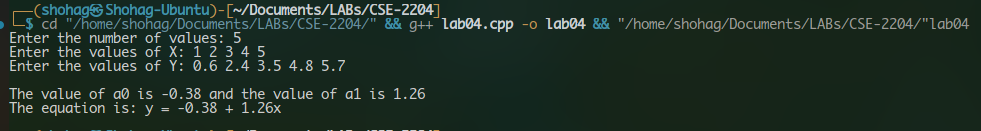
\includegraphics[width=\textwidth]{result.png}
    \caption{Output of the Program}
    \label{fig:result}
\end{figure}

\end{document}